\documentclass{article}
\usepackage{latex-screenshot}
\usepackage{annotation} % Required for inserting images
\addbibresource{../../global_reference.bib}
\usetikzlibrary{patterns}
\newcolumntype{P}[1]{>{\centering\arraybackslash}p{#1}}%center table column elements
\newcolumntype{L}{>{\raggedright\arraybackslash}X}
\hfuzz=80pt
\hbadness=100000000
\begin{document}

\thispagestyle{empty}

\begin{center}
	\centering
	\vspace*{0.08\textheight}

	{\Large\textsc{Personal Annotation Notes} \par}
	\vspace{0.9cm}
  {\LARGE DNA springs project 2026-27 \par}
	\vspace{0.5cm}
	{\normalsize made with great love and curiosity\par}

	\vfill

  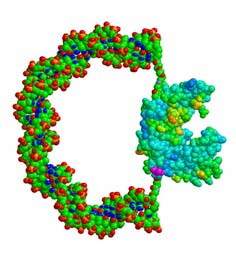
\includegraphics[width=0.3\textwidth]{assets/(cover)DNA springs project 2026-27.jpg}\par

	\vfill

	{\large Ian Poon\par}
	\vspace{0.35cm}
  {\normalsize July 2026\par}
	\vspace{0.9cm}
\end{center}

\newpage

\tableofcontents
\newpage
\begin{abstract}
 just a annotation document... 
\end{abstract}
\section{27/07/2026  TCO ssDNA/PEG5K + Tet sfGFP}

\begin{figure}[H]
  \centering
  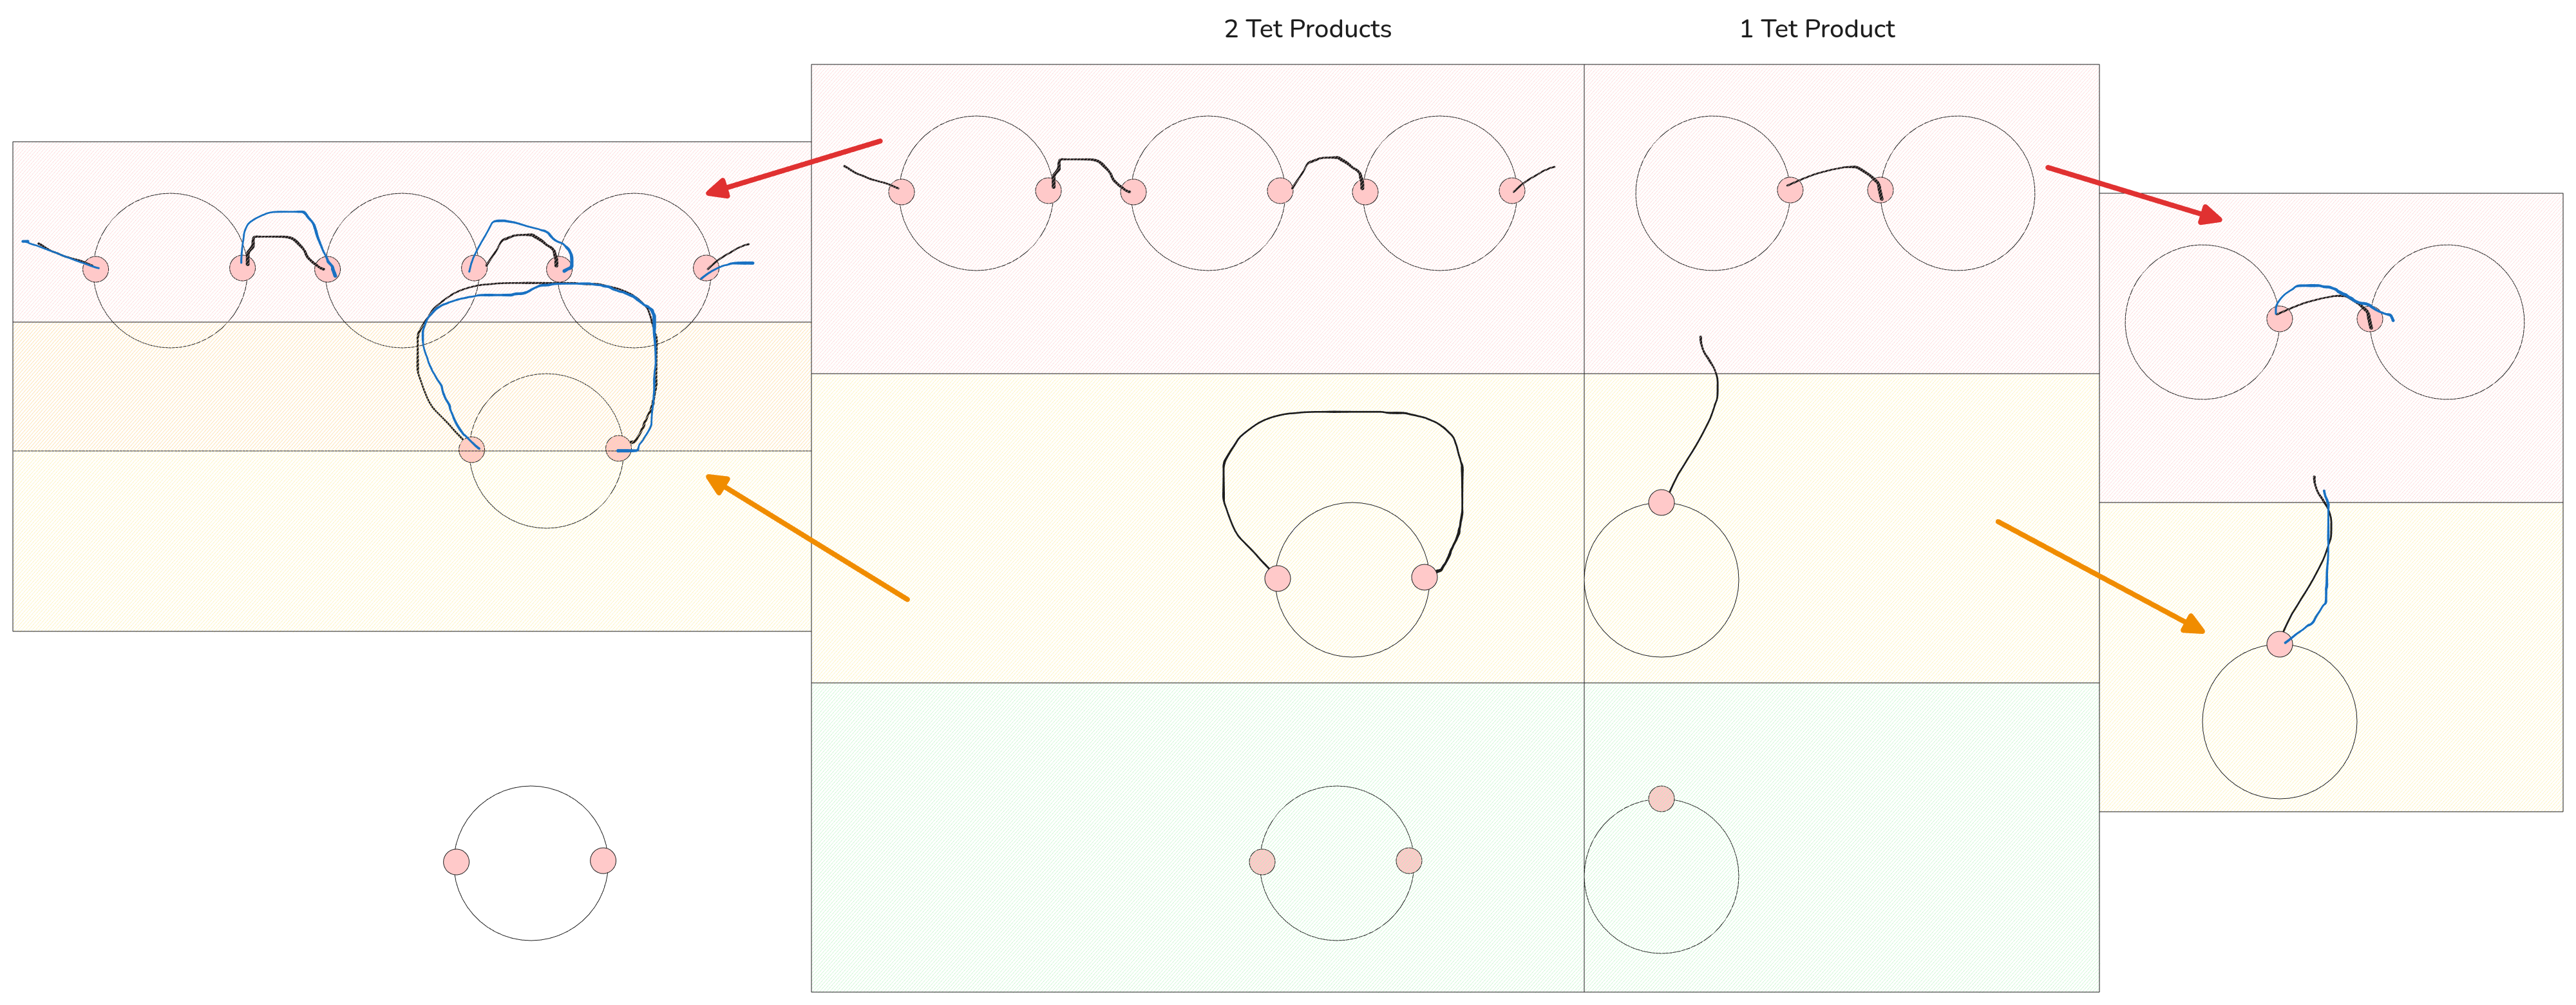
\includegraphics[width=0.5\textwidth]{assets/dna-springs-project-2026-27-2026-07-27-10-36-53.png}
  \caption{}
  \label{fig:dna-springs-project-2026-27-2026-07-27-10-36-53}
\end{figure}

\printbibliography
\end{document}

